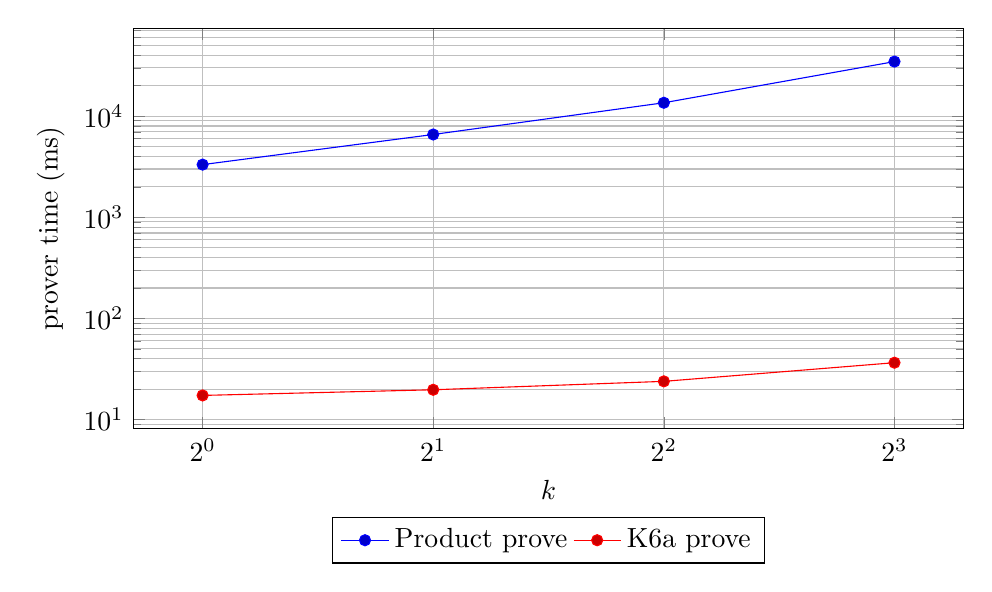
\begin{tikzpicture}
\begin{axis}[
  width=\linewidth,
  height=0.55\linewidth,
  grid=both,
  xmode=log,
  log basis x=2,
  xtick=data,
  xlabel={$k$},
  ylabel={prover time (ms)},
  legend style={at={(0.5,-0.22)},anchor=north,legend columns=2},
  ymode=log,
  log basis y=10
]
\addplot+[mark=*] coordinates {(1,3317.38) (2,6587.36) (4,13561.8) (8,34612.7)};
\addlegendentry{Product prove}
\addplot+[mark=*] coordinates {(1,17.3459) (2,19.7257) (4,23.8886) (8,36.5322)};
\addlegendentry{K6a prove}
\end{axis}
\end{tikzpicture}
